% SC2002 --- Chapter 5: SOLID & Design Principles (0->100 ground-up)
\chapter[SOLID \& Design Principles]{SOLID \& Design Principles: From Code That Works to Code That Lasts}
\label{ch:solid}

\begin{quote}
\emph{``You cannot design well without principles; you cannot follow principles without judgement.''} --- SOLID is five interlocking principles that turn ``it works'' into ``it stays workable.'' Each principle names one way code degrades---and the habit that prevents it.
\end{quote}

\noindent\fbox{\parbox{\dimexpr\linewidth-2\fboxsep-2\fboxrule}{%
\textbf{From zero: built on Ch.~1--4.} Each SOLID principle is motivated from a concrete code smell you have already seen (god class, copy-paste, fragile override). No prior design-principles assumed.}}
\vspace{0.4em}

\section*{Learning Outcomes}
After this chapter you will be able to:
\begin{enumerate}[label=(L\arabic*)]
    \item state each SOLID principle and the symptom it cures (SRP, OCP, LSP, ISP, DIP);
    \item apply cohesion/coupling, DRY, and encapsulation to judge a design;
    \item refactor a god class, a switch-on-type, and a fat interface using SOLID;
    \item explain dependency inversion and how interfaces decouple high-level policy from low-level detail;
    \item trade off principles against simplicity (YAGNI, KISS) and avoid over-engineering.
\end{enumerate}

% ============================================================
\section{Single Responsibility and Open--Closed}
\label{sec:srp-ocp}
\paragraph{SRP---A class should have one reason to change.} A \texttt{Report} that formats, prints, and saves has three reasons to change (layout, printer driver, file format). Split into \texttt{Report}, \texttt{ReportFormatter}, \texttt{ReportPrinter}, \texttt{ReportRepository}---each with high cohesion.

\begin{figure}[h]
\centering
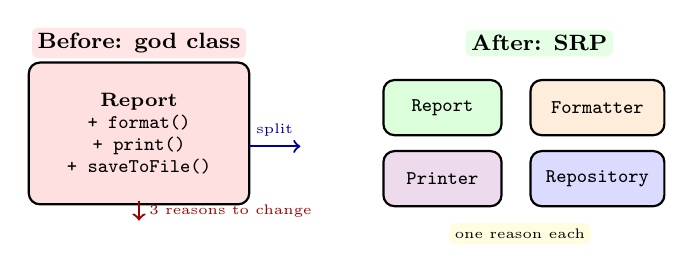
\begin{tikzpicture}[scale=0.82, every node/.style={font=\scriptsize}]
\begin{scope}
\node[font=\footnotesize\bfseries,fill=red!10,rounded corners=2pt,inner sep=2pt] at (1.5,1.6) {Before: god class};
\node[draw,thick,fill=red!12,rounded corners=4pt,minimum width=2.8cm,minimum height=1.8cm,align=center] at (1.5,0.2) {\textbf{Report}\\\texttt{+ format()}\\\texttt{+ print()}\\\texttt{+ saveToFile()}};
\draw[->,thick,red!60!black] (1.5,-0.85) -- (1.5,-1.15) node[midway,right,font=\tiny] {3 reasons to change};
\end{scope}
\draw[->,thick,blue!60!black] (3.2,0.0) -- (4.0,0.0) node[midway,above,font=\tiny] {split};
\begin{scope}[xshift=6.2cm]
\node[font=\footnotesize\bfseries,fill=green!10,rounded corners=2pt,inner sep=2pt] at (1.5,1.6) {After: SRP};
\node[draw,thick,fill=green!14,rounded corners=4pt,minimum width=1.5cm,minimum height=0.7cm] at (0,0.6) {\texttt{Report}};
\node[draw,thick,fill=orange!14,rounded corners=4pt,minimum width=1.7cm,minimum height=0.7cm] at (2.4,0.6) {\texttt{Formatter}};
\node[draw,thick,fill=violet!14,rounded corners=4pt,minimum width=1.5cm,minimum height=0.7cm] at (0,-0.5) {\texttt{Printer}};
\node[draw,thick,fill=blue!14,rounded corners=4pt,minimum width=1.7cm,minimum height=0.7cm] at (2.4,-0.5) {\texttt{Repository}};
\node[font=\tiny,align=center,fill=yellow!12,rounded corners=2pt,inner sep=2pt] at (1.2,-1.35) {one reason each};
\end{scope}
\end{tikzpicture}
\caption{SRP: split a god class so each class has one axis of change.}
\label{fig:srp-split}
\end{figure}

\paragraph{OCP---Open for extension, closed for modification.} New behaviour should be added by adding new code, not editing old code. The mechanism is polymorphism: depend on an abstraction, plug in new implementations.

\begin{lstlisting}[language=Java, caption={OCP via polymorphism---no switch, no edit to add a new shape.}]
// Violates OCP: every new shape edits this method
double area(Object s) {
    if (s instanceof Circle c) return Math.PI*c.r()*c.r();
    if (s instanceof Rectangle r) return r.w()*r.h();
    throw new IllegalArgumentException();
}
// OCP: add a new Shape subtype; AreaCalculator never changes
interface Shape { double area(); }
class Circle implements Shape { double r; public double area(){return Math.PI*r*r;}}
class AreaCalculator { double total(List<Shape> ss){ return ss.stream().mapToDouble(Shape::area).sum();}}
\end{lstlisting}

% --- TikZ 2: OCP extension diagram ---
\begin{figure}[h]
\centering
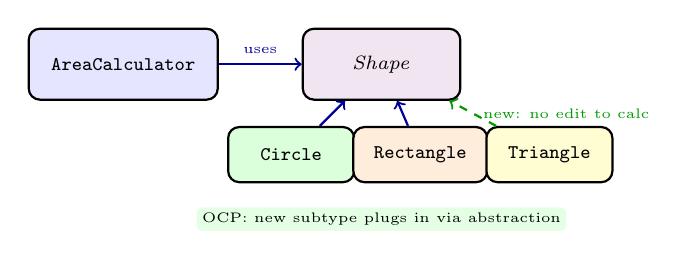
\begin{tikzpicture}[scale=0.82, every node/.style={font=\scriptsize}]
\node[draw,thick,fill=blue!10,rounded corners=4pt,minimum width=2.4cm,minimum height=0.9cm] (calc) at (0,0) {\texttt{AreaCalculator}};
\node[draw,thick,fill=violet!10,rounded corners=4pt,minimum width=2.0cm,minimum height=0.9cm] (shape) at (4.0,0) {\textit{Shape}};
\node[draw,thick,fill=green!14,rounded corners=4pt,minimum width=1.6cm,minimum height=0.7cm] (c) at (2.6,-1.4) {\texttt{Circle}};
\node[draw,thick,fill=orange!14,rounded corners=4pt,minimum width=1.7cm,minimum height=0.7cm] (r) at (4.6,-1.4) {\texttt{Rectangle}};
\node[draw,thick,fill=yellow!18,rounded corners=4pt,minimum width=1.6cm,minimum height=0.7cm] (t) at (6.6,-1.4) {\texttt{Triangle}};
\draw[->,thick,blue!60!black] (calc) -- (shape) node[midway,above,font=\tiny] {uses};
\draw[->,thick,blue!60!black] (c) -- (shape);
\draw[->,thick,blue!60!black] (r) -- (shape);
\draw[->,thick,green!60!black,dashed] (t) -- (shape) node[midway,right,font=\tiny] {new: no edit to calc};
\node[font=\tiny,fill=green!10,rounded corners=2pt,inner sep=2pt] at (4.0,-2.4) {OCP: new subtype plugs in via abstraction};
\end{tikzpicture}
\caption{OCP in structure: \texttt{AreaCalculator} depends on the \texttt{Shape} abstraction; adding \texttt{Triangle} touches no existing class.}
\label{fig:ocp-extension}
\end{figure}

\section{Liskov, Interface Segregation, Dependency Inversion}
\label{sec:lsp-isp-dip}
\paragraph{LSP---Subtypes must be substitutable.} From Ch.~3: overriding must not strengthen preconditions or weaken postconditions. A method expecting \texttt{Rectangle} must work with any subtype. Design hierarchies around behaviour, not data shape.

\paragraph{ISP---Many specific interfaces beat one general one.} A fat interface forces clients to depend on methods they never use. Split it.

\begin{lstlisting}[language=Java, caption={ISP: fat interface vs.\ segregated roles.}]
// Fat: Printer must implement staple() even if it cannot staple
interface Machine { void print(); void scan(); void staple(); }
// Segregated: clients depend only on what they use
interface Printer { void print(); }
interface Scanner { void scan(); }
interface Stapler { void staple(); }
class SimplePrinter implements Printer { public void print(){ /*...*/ } }
\end{lstlisting}

\paragraph{DIP---Depend on abstractions, not concretions.} High-level policy (e.g., \texttt{CheckoutService}) should not depend on low-level detail (\texttt{MySQLBookRepository}); both should depend on an abstraction (\texttt{BookRepository} interface). This inverts the naive dependency direction.

% --- TikZ 3: DIP inversion ---
\begin{figure}[h]
\centering
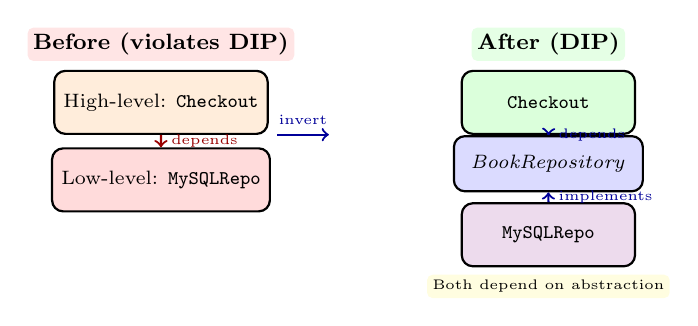
\begin{tikzpicture}[scale=0.82, every node/.style={font=\scriptsize}]
\begin{scope}
\node[font=\footnotesize\bfseries,fill=red!10,rounded corners=2pt,inner sep=2pt] at (1.6,1.4) {Before (violates DIP)};
\node[draw,thick,fill=orange!14,rounded corners=4pt,minimum width=2.2cm,minimum height=0.8cm] (hi1) at (1.6,0.5) {High-level: \texttt{Checkout}};
\node[draw,thick,fill=red!14,rounded corners=4pt,minimum width=2.2cm,minimum height=0.8cm] (lo1) at (1.6,-0.7) {Low-level: \texttt{MySQLRepo}};
\draw[->,thick,red!60!black] (hi1) -- (lo1) node[midway,right,font=\tiny] {depends};
\end{scope}
\draw[->,thick,blue!60!black] (3.4,0) -- (4.2,0) node[midway,above,font=\tiny] {invert};
\begin{scope}[xshift=6.0cm]
\node[font=\footnotesize\bfseries,fill=green!10,rounded corners=2pt,inner sep=2pt] at (1.6,1.4) {After (DIP)};
\node[draw,thick,fill=green!14,rounded corners=4pt,minimum width=2.2cm,minimum height=0.8cm] (hi2) at (1.6,0.5) {\texttt{Checkout}};
\node[draw,thick,fill=blue!14,rounded corners=4pt,minimum width=2.4cm,minimum height=0.7cm] (abs) at (1.6,-0.45) {\textit{BookRepository}};
\node[draw,thick,fill=violet!14,rounded corners=4pt,minimum width=2.2cm,minimum height=0.8cm] (lo2) at (1.6,-1.55) {\texttt{MySQLRepo}};
\draw[->,thick,blue!60!black] (hi2) -- (abs) node[midway,right,font=\tiny] {depends};
\draw[->,thick,blue!60!black] (lo2) -- (abs) node[midway,right,font=\tiny] {implements};
\node[font=\tiny,fill=yellow!12,rounded corners=2pt,inner sep=2pt] at (1.6,-2.35) {Both depend on abstraction};
\end{scope}
\end{tikzpicture}
\caption{DIP: introduce an abstraction so high-level policy does not depend on low-level detail; both depend on the interface.}
\label{fig:dip-inversion}
\end{figure}

\begin{remark}[SOLID together]
SRP and ISP split things that change for different reasons; OCP and DIP make extension cheap; LSP keeps hierarchies honest. Apply all five lightly---over-splitting creates indirection without value (YAGNI/KISS). Let the next requirement, not speculation, drive the split.
\end{remark}

\section{How SOLID Feels in Practice: Smells and Heuristics}
\label{sec:solid-practice}
SOLID is easier to apply when you can name the smell it cures.

\begin{center}
\small
\begin{tabular}{lll}
\toprule
Smell & Principle it violates & Fix \\
\midrule
God class / long method & SRP & Extract class/method \\
Switch on type & OCP & Strategy / polymorphism \\
Subclass throws on super method & LSP & Re-hierarchy or composition \\
Fat interface, forced empty methods & ISP & Split interfaces \\
\texttt{new} everywhere, hard to test & DIP & Factory + constructor injection \\
\bottomrule
\end{tabular}
\end{center}

\paragraph{Heuristics that reinforce SOLID.} DRY (don't repeat yourself) pushes toward abstraction; YAGNI (you aren't gonna need it) pulls back from speculation---apply SOLID at the second variant, not the first guess. Encapsulation (Ch.~2) and favouring composition over inheritance (Ch.~3) are the mechanisms SOLID builds on.

\begin{lstlisting}[language=Java, caption={DIP + injection makes testing trivial (preview of Ch.~8).}]
class CheckoutService {
    private final BookRepository repo; // abstraction, not MySQLRepo
    private final PaymentGateway gateway;
    public CheckoutService(BookRepository repo, PaymentGateway gw){
        this.repo = repo; this.gateway = gw; // constructor injection
    }
    public Receipt checkout(String memberId, String bookId){
        Book b = repo.findById(bookId).orElseThrow();
        // ... policy + payment via gateway
        return new Receipt(b);
    }
}
// Test injects in-memory fakes: new CheckoutService(new InMemoryRepo(), new FakeGateway())
\end{lstlisting}

\paragraph{When not to SOLID.} A one-off script, a prototype, or a module with one known variant does not need five interfaces. Let the pain (second variant, painful test, painful change) justify the abstraction.

\subsection{From Principles to Code Reviews}
A practical review checklist derived from SOLID:
\begin{enumerate}[itemsep=0.2em]
    \item Does this class have a one-sentence responsibility? If not, split (SRP).
    \item Would a new variant require editing this file? If yes, introduce an abstraction (OCP/DIP).
    \item Does any subclass break a supertype test? If yes, fix the hierarchy (LSP).
    \item Does any client implement methods it never calls? If yes, split the interface (ISP).
    \item Does high-level code mention a low-level concrete name? If yes, invert via interface (DIP).
\end{enumerate}
Apply the checklist on every pull request; the cost is minutes, the saving is weeks of coupled changes. Record the decision (ADR) when you introduce an abstraction so future readers know \emph{why} the seam exists.

\paragraph{Metrics that correlate.} Tools like SonarQube flag god classes (SRP), package cycles (DIP), and duplicate switches (OCP). Treat metric warnings as prompts for judgement, not automatic refactor triggers---confirm with the smell table above before changing code.

\subsection{Dependency Inversion in Layers}
In a layered architecture (UI $\to$ Service $\to$ Repository $\to$ DB), naive dependencies point downwards: Service knows MySQL. DIP flips the boundary: Service owns the \texttt{Repository} interface in \emph{its} package; the MySQL adapter in the infrastructure package implements it. The dependency arrow now points \emph{inward} toward policy, not outward toward detail---high-level policy is independent of storage choice and can be tested with an in-memory fake.

\begin{center}
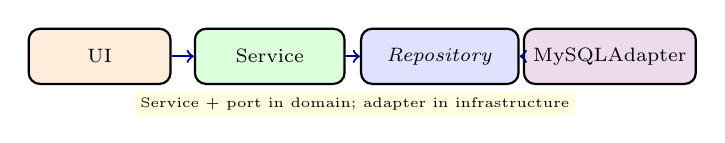
\begin{tikzpicture}[scale=0.80, every node/.style={font=\scriptsize}]
\node[draw,thick,fill=orange!14,rounded corners=4pt,minimum width=1.8cm,minimum height=0.7cm] (ui) at (0,0) {UI};
\node[draw,thick,fill=green!14,rounded corners=4pt,minimum width=1.9cm,minimum height=0.7cm] (svc) at (2.7,0) {Service};
\node[draw,thick,fill=blue!12,rounded corners=4pt,minimum width=2.0cm,minimum height=0.7cm] (port) at (5.4,0) {\textit{Repository}};
\node[draw,thick,fill=violet!14,rounded corners=4pt,minimum width=1.9cm,minimum height=0.7cm] (ad) at (8.1,0) {MySQLAdapter};
\draw[->,thick,blue!60!black] (ui)--(svc); \draw[->,thick,blue!60!black] (svc)--(port); \draw[->,thick,blue!60!black] (ad)--(port);
\node[font=\tiny,fill=yellow!12,rounded corners=2pt,inner sep=2pt] at (4.05,-0.75) {Service + port in domain; adapter in infrastructure};
\end{tikzpicture}
\end{center}

\section{Chapter Notes}
SOLID was named by Martin (2000) synthesising earlier work (Liskov 1987 for LSP, Martin for DIP/ISP). Effective Java and Clean Architecture (Martin) show pragmatic trade-offs. Coupling/cohesion, DRY, and YAGNI are complementary heuristics from Constantine, Hunt \& Thomas, and Beck.

\section{Exercises}
\label{sec:ch05-exercises}
\begin{enumerate}[label=E5.\arabic*, leftmargin=*, itemsep=0.8em]
    \item \textbf{SRP refactor.} \texttt{Order} currently validates, calculates total, formats receipt, and saves to DB. Identify each reason to change, split into cohesive classes, and show the new dependencies.
    \item \textbf{OCP without switch.} A \texttt{PaymentProcessor} switches on \texttt{type=="CASH"/"CARD"/"PAYNOW"}. Refactor to a \texttt{PaymentMethod} hierarchy so adding \texttt{CRYPTO} needs no edit to \texttt{PaymentProcessor}. Draw the class diagram.
    \item \textbf{LSP audit.} \texttt{ReadOnlyBook extends Book} but throws on \texttt{markBorrowed()}. Explain the LSP violation, give a failing client snippet, and propose a hierarchy that honours LSP.
    \item \textbf{ISP split.} Interface \texttt{Worker \{ work(); eat(); sleep(); \}} is implemented by \texttt{Robot} (which does not eat/sleep). Apply ISP, show the segregated interfaces, and explain how client coupling drops.
    \item \textbf{DIP wiring.} \texttt{NotificationService} currently constructs \texttt{new EmailSender()} internally. Apply DIP with a \texttt{Sender} interface, show constructor injection, and explain how testing benefits (mock sender).
\end{enumerate}
% End of Chapter 5
